\documentclass[12pt, a4paper, oneside]{report}
\usepackage[lmargin=0.75in, rmargin=0.75in, tmargin=0.5in, bmargin=0.5in]{geometry}


\usepackage[english]{babel}
\usepackage[utf8]{inputenc}


\usepackage{graphicx}
\usepackage{subfig}
% \usepackage{cleveref}

\usepackage{caption}


\usepackage{lipsum}
\usepackage{titlesec}

\titleformat{\chapter}[display]
  {\normalfont\bfseries}{}{0pt}{\Huge}
  
\usepackage{enumitem}

\usepackage{url} 

\usepackage{amsmath}    

\usepackage{listings}          % for creating language style
 %%%%%%%%%%%%%%%%%%%%%%%%%%%%%%%%%%%%%%%%%%%%%%%%%%%%%%%%%%%%%%%%%%%%%%%%%%%%%%%% 
%%% ~ Arduino Language - Arduino IDE Colors ~                                  %%%
%%%                                                                            %%%
%%% Kyle Rocha-Brownell | 10/2/2017 | No Licence                               %%%
%%% -------------------------------------------------------------------------- %%%
%%%                                                                            %%%
%%% Place this file in your working directory (next to the latex file you're   %%%
%%% working on).  To add it to your project, place:                            %%%
%%%     %%%%%%%%%%%%%%%%%%%%%%%%%%%%%%%%%%%%%%%%%%%%%%%%%%%%%%%%%%%%%%%%%%%%%%%%%%%%%%%% 
%%% ~ Arduino Language - Arduino IDE Colors ~                                  %%%
%%%                                                                            %%%
%%% Kyle Rocha-Brownell | 10/2/2017 | No Licence                               %%%
%%% -------------------------------------------------------------------------- %%%
%%%                                                                            %%%
%%% Place this file in your working directory (next to the latex file you're   %%%
%%% working on).  To add it to your project, place:                            %%%
%%%     %%%%%%%%%%%%%%%%%%%%%%%%%%%%%%%%%%%%%%%%%%%%%%%%%%%%%%%%%%%%%%%%%%%%%%%%%%%%%%%% 
%%% ~ Arduino Language - Arduino IDE Colors ~                                  %%%
%%%                                                                            %%%
%%% Kyle Rocha-Brownell | 10/2/2017 | No Licence                               %%%
%%% -------------------------------------------------------------------------- %%%
%%%                                                                            %%%
%%% Place this file in your working directory (next to the latex file you're   %%%
%%% working on).  To add it to your project, place:                            %%%
%%%    \input{arduinoLanguage.tex}                                             %%%
%%% somewhere before \begin{document} in your latex file.                      %%%
%%%                                                                            %%%
%%% In your document, place your arduino code between:                         %%%
%%%   \begin{lstlisting}[language=Arduino]                                     %%%
%%% and:                                                                       %%%
%%%   \end{lstlisting}                                                         %%%
%%%                                                                            %%%
%%% Or create your own style to add non-built-in functions and variables.      %%%
%%%                                                                            %%%
 %%%%%%%%%%%%%%%%%%%%%%%%%%%%%%%%%%%%%%%%%%%%%%%%%%%%%%%%%%%%%%%%%%%%%%%%%%%%%%%% 

 \usepackage{color}
 \usepackage{listings}    
 \usepackage{courier}
 
 %%% Define Custom IDE Colors %%%
 \definecolor{arduinoGreen}    {rgb} {0.17, 0.43, 0.01}
 \definecolor{arduinoGrey}     {rgb} {0.47, 0.47, 0.33}
 \definecolor{arduinoOrange}   {rgb} {0.8 , 0.4 , 0   }
 \definecolor{arduinoBlue}     {rgb} {0.01, 0.61, 0.98}
 \definecolor{arduinoDarkBlue} {rgb} {0.0 , 0.2 , 0.5 }
 
 %%% Define Arduino Language %%%
 \lstdefinelanguage{Arduino}{
   language=C++, % begin with default C++ settings 
 %
 %
   %%% Keyword Color Group 1 %%%  (called KEYWORD3 by arduino)
   keywordstyle=\color{arduinoGreen},   
   deletekeywords={  % remove all arduino keywords that might be in c++
                 break, case, override, final, continue, default, do, else, for, 
                 if, return, goto, switch, throw, try, while, setup, loop, export, 
                 not, or, and, xor, include, define, elif, else, error, if, ifdef, 
                 ifndef, pragma, warning,
                 HIGH, LOW, INPUT, INPUT_PULLUP, OUTPUT, DEC, BIN, HEX, OCT, PI, 
                 HALF_PI, TWO_PI, LSBFIRST, MSBFIRST, CHANGE, FALLING, RISING, 
                 DEFAULT, EXTERNAL, INTERNAL, INTERNAL1V1, INTERNAL2V56, LED_BUILTIN, 
                 LED_BUILTIN_RX, LED_BUILTIN_TX, DIGITAL_MESSAGE, FIRMATA_STRING, 
                 ANALOG_MESSAGE, REPORT_DIGITAL, REPORT_ANALOG, SET_PIN_MODE, 
                 SYSTEM_RESET, SYSEX_START, auto, int8_t, int16_t, int32_t, int64_t, 
                 uint8_t, uint16_t, uint32_t, uint64_t, char16_t, char32_t, operator, 
                 enum, delete, bool, boolean, byte, char, const, false, float, double, 
                 null, NULL, int, long, new, private, protected, public, short, 
                 signed, static, volatile, String, void, true, unsigned, word, array, 
                 sizeof, dynamic_cast, typedef, const_cast, struct, static_cast, union, 
                 friend, extern, class, reinterpret_cast, register, explicit, inline, 
                 _Bool, complex, _Complex, _Imaginary, atomic_bool, atomic_char, 
                 atomic_schar, atomic_uchar, atomic_short, atomic_ushort, atomic_int, 
                 atomic_uint, atomic_long, atomic_ulong, atomic_llong, atomic_ullong, 
                 virtual, PROGMEM,
                 Serial, Serial1, Serial2, Serial3, SerialUSB, Keyboard, Mouse,
                 abs, acos, asin, atan, atan2, ceil, constrain, cos, degrees, exp, 
                 floor, log, map, max, min, radians, random, randomSeed, round, sin, 
                 sq, sqrt, tan, pow, bitRead, bitWrite, bitSet, bitClear, bit, 
                 highByte, lowByte, analogReference, analogRead, 
                 analogReadResolution, analogWrite, analogWriteResolution, 
                 attachInterrupt, detachInterrupt, digitalPinToInterrupt, delay, 
                 delayMicroseconds, digitalWrite, digitalRead, interrupts, millis, 
                 micros, noInterrupts, noTone, pinMode, pulseIn, pulseInLong, shiftIn, 
                 shiftOut, tone, yield, Stream, begin, end, peek, read, print, 
                 println, available, availableForWrite, flush, setTimeout, find, 
                 findUntil, parseInt, parseFloat, readBytes, readBytesUntil, readString, 
                 readStringUntil, trim, toUpperCase, toLowerCase, charAt, compareTo, 
                 concat, endsWith, startsWith, equals, equalsIgnoreCase, getBytes, 
                 indexOf, lastIndexOf, length, replace, setCharAt, substring, 
                 toCharArray, toInt, press, release, releaseAll, accept, click, move, 
                 isPressed, isAlphaNumeric, isAlpha, isAscii, isWhitespace, isControl, 
                 isDigit, isGraph, isLowerCase, isPrintable, isPunct, isSpace, 
                 isUpperCase, isHexadecimalDigit, 
                 }, 
   morekeywords={   % add arduino structures to group 1
                 break, case, override, final, continue, default, do, else, for, 
                 if, return, goto, switch, throw, try, while, setup, loop, export, 
                 not, or, and, xor, include, define, elif, else, error, if, ifdef, 
                 ifndef, pragma, warning,
                 }, 
 % 
 %
   %%% Keyword Color Group 2 %%%  (called LITERAL1 by arduino)
   keywordstyle=[2]\color{arduinoBlue},   
   keywords=[2]{   % add variables and dataTypes as 2nd group  
                 HIGH, LOW, INPUT, INPUT_PULLUP, OUTPUT, DEC, BIN, HEX, OCT, PI, 
                 HALF_PI, TWO_PI, LSBFIRST, MSBFIRST, CHANGE, FALLING, RISING, 
                 DEFAULT, EXTERNAL, INTERNAL, INTERNAL1V1, INTERNAL2V56, LED_BUILTIN, 
                 LED_BUILTIN_RX, LED_BUILTIN_TX, DIGITAL_MESSAGE, FIRMATA_STRING, 
                 ANALOG_MESSAGE, REPORT_DIGITAL, REPORT_ANALOG, SET_PIN_MODE, 
                 SYSTEM_RESET, SYSEX_START, auto, int8_t, int16_t, int32_t, int64_t, 
                 uint8_t, uint16_t, uint32_t, uint64_t, char16_t, char32_t, operator, 
                 enum, delete, bool, boolean, byte, char, const, false, float, double, 
                 null, NULL, int, long, new, private, protected, public, short, 
                 signed, static, volatile, String, void, true, unsigned, word, array, 
                 sizeof, dynamic_cast, typedef, const_cast, struct, static_cast, union, 
                 friend, extern, class, reinterpret_cast, register, explicit, inline, 
                 _Bool, complex, _Complex, _Imaginary, atomic_bool, atomic_char, 
                 atomic_schar, atomic_uchar, atomic_short, atomic_ushort, atomic_int, 
                 atomic_uint, atomic_long, atomic_ulong, atomic_llong, atomic_ullong, 
                 virtual, PROGMEM,
                 },  
 % 
 %
   %%% Keyword Color Group 3 %%%  (called KEYWORD1 by arduino)
   keywordstyle=[3]\bfseries\color{arduinoOrange},
   keywords=[3]{  % add built-in functions as a 3rd group
                 Serial, Serial1, Serial2, Serial3, SerialUSB, Keyboard, Mouse,
                 },      
 %
 %
   %%% Keyword Color Group 4 %%%  (called KEYWORD2 by arduino)
   keywordstyle=[4]\color{arduinoOrange},
   keywords=[4]{  % add more built-in functions as a 4th group
                 abs, acos, asin, atan, atan2, ceil, constrain, cos, degrees, exp, 
                 floor, log, map, max, min, radians, random, randomSeed, round, sin, 
                 sq, sqrt, tan, pow, bitRead, bitWrite, bitSet, bitClear, bit, 
                 highByte, lowByte, analogReference, analogRead, 
                 analogReadResolution, analogWrite, analogWriteResolution, 
                 attachInterrupt, detachInterrupt, digitalPinToInterrupt, delay, 
                 delayMicroseconds, digitalWrite, digitalRead, interrupts, millis, 
                 micros, noInterrupts, noTone, pinMode, pulseIn, pulseInLong, shiftIn, 
                 shiftOut, tone, yield, Stream, begin, end, peek, read, print, 
                 println, available, availableForWrite, flush, setTimeout, find, 
                 findUntil, parseInt, parseFloat, readBytes, readBytesUntil, readString, 
                 readStringUntil, trim, toUpperCase, toLowerCase, charAt, compareTo, 
                 concat, endsWith, startsWith, equals, equalsIgnoreCase, getBytes, 
                 indexOf, lastIndexOf, length, replace, setCharAt, substring, 
                 toCharArray, toInt, press, release, releaseAll, accept, click, move, 
                 isPressed, isAlphaNumeric, isAlpha, isAscii, isWhitespace, isControl, 
                 isDigit, isGraph, isLowerCase, isPrintable, isPunct, isSpace, 
                 isUpperCase, isHexadecimalDigit, 
                 },      
 %
 %
   %%% Set Other Colors %%%
   stringstyle=\color{arduinoDarkBlue},    
   commentstyle=\color{arduinoGrey},    
 %          
 %   
   %%%% Line Numbering %%%%
   numbers=left,                    
   numbersep=5pt,                   
   numberstyle=\color{arduinoGrey},    
   %stepnumber=2,                      % show every 2 line numbers
 %
 %
   %%%% Code Box Style %%%%
   breaklines=true,                    % wordwrapping
   tabsize=2,         
   basicstyle=\ttfamily  
 }                                             %%%
%%% somewhere before \begin{document} in your latex file.                      %%%
%%%                                                                            %%%
%%% In your document, place your arduino code between:                         %%%
%%%   \begin{lstlisting}[language=Arduino]                                     %%%
%%% and:                                                                       %%%
%%%   \end{lstlisting}                                                         %%%
%%%                                                                            %%%
%%% Or create your own style to add non-built-in functions and variables.      %%%
%%%                                                                            %%%
 %%%%%%%%%%%%%%%%%%%%%%%%%%%%%%%%%%%%%%%%%%%%%%%%%%%%%%%%%%%%%%%%%%%%%%%%%%%%%%%% 

 \usepackage{color}
 \usepackage{listings}    
 \usepackage{courier}
 
 %%% Define Custom IDE Colors %%%
 \definecolor{arduinoGreen}    {rgb} {0.17, 0.43, 0.01}
 \definecolor{arduinoGrey}     {rgb} {0.47, 0.47, 0.33}
 \definecolor{arduinoOrange}   {rgb} {0.8 , 0.4 , 0   }
 \definecolor{arduinoBlue}     {rgb} {0.01, 0.61, 0.98}
 \definecolor{arduinoDarkBlue} {rgb} {0.0 , 0.2 , 0.5 }
 
 %%% Define Arduino Language %%%
 \lstdefinelanguage{Arduino}{
   language=C++, % begin with default C++ settings 
 %
 %
   %%% Keyword Color Group 1 %%%  (called KEYWORD3 by arduino)
   keywordstyle=\color{arduinoGreen},   
   deletekeywords={  % remove all arduino keywords that might be in c++
                 break, case, override, final, continue, default, do, else, for, 
                 if, return, goto, switch, throw, try, while, setup, loop, export, 
                 not, or, and, xor, include, define, elif, else, error, if, ifdef, 
                 ifndef, pragma, warning,
                 HIGH, LOW, INPUT, INPUT_PULLUP, OUTPUT, DEC, BIN, HEX, OCT, PI, 
                 HALF_PI, TWO_PI, LSBFIRST, MSBFIRST, CHANGE, FALLING, RISING, 
                 DEFAULT, EXTERNAL, INTERNAL, INTERNAL1V1, INTERNAL2V56, LED_BUILTIN, 
                 LED_BUILTIN_RX, LED_BUILTIN_TX, DIGITAL_MESSAGE, FIRMATA_STRING, 
                 ANALOG_MESSAGE, REPORT_DIGITAL, REPORT_ANALOG, SET_PIN_MODE, 
                 SYSTEM_RESET, SYSEX_START, auto, int8_t, int16_t, int32_t, int64_t, 
                 uint8_t, uint16_t, uint32_t, uint64_t, char16_t, char32_t, operator, 
                 enum, delete, bool, boolean, byte, char, const, false, float, double, 
                 null, NULL, int, long, new, private, protected, public, short, 
                 signed, static, volatile, String, void, true, unsigned, word, array, 
                 sizeof, dynamic_cast, typedef, const_cast, struct, static_cast, union, 
                 friend, extern, class, reinterpret_cast, register, explicit, inline, 
                 _Bool, complex, _Complex, _Imaginary, atomic_bool, atomic_char, 
                 atomic_schar, atomic_uchar, atomic_short, atomic_ushort, atomic_int, 
                 atomic_uint, atomic_long, atomic_ulong, atomic_llong, atomic_ullong, 
                 virtual, PROGMEM,
                 Serial, Serial1, Serial2, Serial3, SerialUSB, Keyboard, Mouse,
                 abs, acos, asin, atan, atan2, ceil, constrain, cos, degrees, exp, 
                 floor, log, map, max, min, radians, random, randomSeed, round, sin, 
                 sq, sqrt, tan, pow, bitRead, bitWrite, bitSet, bitClear, bit, 
                 highByte, lowByte, analogReference, analogRead, 
                 analogReadResolution, analogWrite, analogWriteResolution, 
                 attachInterrupt, detachInterrupt, digitalPinToInterrupt, delay, 
                 delayMicroseconds, digitalWrite, digitalRead, interrupts, millis, 
                 micros, noInterrupts, noTone, pinMode, pulseIn, pulseInLong, shiftIn, 
                 shiftOut, tone, yield, Stream, begin, end, peek, read, print, 
                 println, available, availableForWrite, flush, setTimeout, find, 
                 findUntil, parseInt, parseFloat, readBytes, readBytesUntil, readString, 
                 readStringUntil, trim, toUpperCase, toLowerCase, charAt, compareTo, 
                 concat, endsWith, startsWith, equals, equalsIgnoreCase, getBytes, 
                 indexOf, lastIndexOf, length, replace, setCharAt, substring, 
                 toCharArray, toInt, press, release, releaseAll, accept, click, move, 
                 isPressed, isAlphaNumeric, isAlpha, isAscii, isWhitespace, isControl, 
                 isDigit, isGraph, isLowerCase, isPrintable, isPunct, isSpace, 
                 isUpperCase, isHexadecimalDigit, 
                 }, 
   morekeywords={   % add arduino structures to group 1
                 break, case, override, final, continue, default, do, else, for, 
                 if, return, goto, switch, throw, try, while, setup, loop, export, 
                 not, or, and, xor, include, define, elif, else, error, if, ifdef, 
                 ifndef, pragma, warning,
                 }, 
 % 
 %
   %%% Keyword Color Group 2 %%%  (called LITERAL1 by arduino)
   keywordstyle=[2]\color{arduinoBlue},   
   keywords=[2]{   % add variables and dataTypes as 2nd group  
                 HIGH, LOW, INPUT, INPUT_PULLUP, OUTPUT, DEC, BIN, HEX, OCT, PI, 
                 HALF_PI, TWO_PI, LSBFIRST, MSBFIRST, CHANGE, FALLING, RISING, 
                 DEFAULT, EXTERNAL, INTERNAL, INTERNAL1V1, INTERNAL2V56, LED_BUILTIN, 
                 LED_BUILTIN_RX, LED_BUILTIN_TX, DIGITAL_MESSAGE, FIRMATA_STRING, 
                 ANALOG_MESSAGE, REPORT_DIGITAL, REPORT_ANALOG, SET_PIN_MODE, 
                 SYSTEM_RESET, SYSEX_START, auto, int8_t, int16_t, int32_t, int64_t, 
                 uint8_t, uint16_t, uint32_t, uint64_t, char16_t, char32_t, operator, 
                 enum, delete, bool, boolean, byte, char, const, false, float, double, 
                 null, NULL, int, long, new, private, protected, public, short, 
                 signed, static, volatile, String, void, true, unsigned, word, array, 
                 sizeof, dynamic_cast, typedef, const_cast, struct, static_cast, union, 
                 friend, extern, class, reinterpret_cast, register, explicit, inline, 
                 _Bool, complex, _Complex, _Imaginary, atomic_bool, atomic_char, 
                 atomic_schar, atomic_uchar, atomic_short, atomic_ushort, atomic_int, 
                 atomic_uint, atomic_long, atomic_ulong, atomic_llong, atomic_ullong, 
                 virtual, PROGMEM,
                 },  
 % 
 %
   %%% Keyword Color Group 3 %%%  (called KEYWORD1 by arduino)
   keywordstyle=[3]\bfseries\color{arduinoOrange},
   keywords=[3]{  % add built-in functions as a 3rd group
                 Serial, Serial1, Serial2, Serial3, SerialUSB, Keyboard, Mouse,
                 },      
 %
 %
   %%% Keyword Color Group 4 %%%  (called KEYWORD2 by arduino)
   keywordstyle=[4]\color{arduinoOrange},
   keywords=[4]{  % add more built-in functions as a 4th group
                 abs, acos, asin, atan, atan2, ceil, constrain, cos, degrees, exp, 
                 floor, log, map, max, min, radians, random, randomSeed, round, sin, 
                 sq, sqrt, tan, pow, bitRead, bitWrite, bitSet, bitClear, bit, 
                 highByte, lowByte, analogReference, analogRead, 
                 analogReadResolution, analogWrite, analogWriteResolution, 
                 attachInterrupt, detachInterrupt, digitalPinToInterrupt, delay, 
                 delayMicroseconds, digitalWrite, digitalRead, interrupts, millis, 
                 micros, noInterrupts, noTone, pinMode, pulseIn, pulseInLong, shiftIn, 
                 shiftOut, tone, yield, Stream, begin, end, peek, read, print, 
                 println, available, availableForWrite, flush, setTimeout, find, 
                 findUntil, parseInt, parseFloat, readBytes, readBytesUntil, readString, 
                 readStringUntil, trim, toUpperCase, toLowerCase, charAt, compareTo, 
                 concat, endsWith, startsWith, equals, equalsIgnoreCase, getBytes, 
                 indexOf, lastIndexOf, length, replace, setCharAt, substring, 
                 toCharArray, toInt, press, release, releaseAll, accept, click, move, 
                 isPressed, isAlphaNumeric, isAlpha, isAscii, isWhitespace, isControl, 
                 isDigit, isGraph, isLowerCase, isPrintable, isPunct, isSpace, 
                 isUpperCase, isHexadecimalDigit, 
                 },      
 %
 %
   %%% Set Other Colors %%%
   stringstyle=\color{arduinoDarkBlue},    
   commentstyle=\color{arduinoGrey},    
 %          
 %   
   %%%% Line Numbering %%%%
   numbers=left,                    
   numbersep=5pt,                   
   numberstyle=\color{arduinoGrey},    
   %stepnumber=2,                      % show every 2 line numbers
 %
 %
   %%%% Code Box Style %%%%
   breaklines=true,                    % wordwrapping
   tabsize=2,         
   basicstyle=\ttfamily  
 }                                             %%%
%%% somewhere before \begin{document} in your latex file.                      %%%
%%%                                                                            %%%
%%% In your document, place your arduino code between:                         %%%
%%%   \begin{lstlisting}[language=Arduino]                                     %%%
%%% and:                                                                       %%%
%%%   \end{lstlisting}                                                         %%%
%%%                                                                            %%%
%%% Or create your own style to add non-built-in functions and variables.      %%%
%%%                                                                            %%%
 %%%%%%%%%%%%%%%%%%%%%%%%%%%%%%%%%%%%%%%%%%%%%%%%%%%%%%%%%%%%%%%%%%%%%%%%%%%%%%%% 

 \usepackage{color}
 \usepackage{listings}    
 \usepackage{courier}
 
 %%% Define Custom IDE Colors %%%
 \definecolor{arduinoGreen}    {rgb} {0.17, 0.43, 0.01}
 \definecolor{arduinoGrey}     {rgb} {0.47, 0.47, 0.33}
 \definecolor{arduinoOrange}   {rgb} {0.8 , 0.4 , 0   }
 \definecolor{arduinoBlue}     {rgb} {0.01, 0.61, 0.98}
 \definecolor{arduinoDarkBlue} {rgb} {0.0 , 0.2 , 0.5 }
 
 %%% Define Arduino Language %%%
 \lstdefinelanguage{Arduino}{
   language=C++, % begin with default C++ settings 
 %
 %
   %%% Keyword Color Group 1 %%%  (called KEYWORD3 by arduino)
   keywordstyle=\color{arduinoGreen},   
   deletekeywords={  % remove all arduino keywords that might be in c++
                 break, case, override, final, continue, default, do, else, for, 
                 if, return, goto, switch, throw, try, while, setup, loop, export, 
                 not, or, and, xor, include, define, elif, else, error, if, ifdef, 
                 ifndef, pragma, warning,
                 HIGH, LOW, INPUT, INPUT_PULLUP, OUTPUT, DEC, BIN, HEX, OCT, PI, 
                 HALF_PI, TWO_PI, LSBFIRST, MSBFIRST, CHANGE, FALLING, RISING, 
                 DEFAULT, EXTERNAL, INTERNAL, INTERNAL1V1, INTERNAL2V56, LED_BUILTIN, 
                 LED_BUILTIN_RX, LED_BUILTIN_TX, DIGITAL_MESSAGE, FIRMATA_STRING, 
                 ANALOG_MESSAGE, REPORT_DIGITAL, REPORT_ANALOG, SET_PIN_MODE, 
                 SYSTEM_RESET, SYSEX_START, auto, int8_t, int16_t, int32_t, int64_t, 
                 uint8_t, uint16_t, uint32_t, uint64_t, char16_t, char32_t, operator, 
                 enum, delete, bool, boolean, byte, char, const, false, float, double, 
                 null, NULL, int, long, new, private, protected, public, short, 
                 signed, static, volatile, String, void, true, unsigned, word, array, 
                 sizeof, dynamic_cast, typedef, const_cast, struct, static_cast, union, 
                 friend, extern, class, reinterpret_cast, register, explicit, inline, 
                 _Bool, complex, _Complex, _Imaginary, atomic_bool, atomic_char, 
                 atomic_schar, atomic_uchar, atomic_short, atomic_ushort, atomic_int, 
                 atomic_uint, atomic_long, atomic_ulong, atomic_llong, atomic_ullong, 
                 virtual, PROGMEM,
                 Serial, Serial1, Serial2, Serial3, SerialUSB, Keyboard, Mouse,
                 abs, acos, asin, atan, atan2, ceil, constrain, cos, degrees, exp, 
                 floor, log, map, max, min, radians, random, randomSeed, round, sin, 
                 sq, sqrt, tan, pow, bitRead, bitWrite, bitSet, bitClear, bit, 
                 highByte, lowByte, analogReference, analogRead, 
                 analogReadResolution, analogWrite, analogWriteResolution, 
                 attachInterrupt, detachInterrupt, digitalPinToInterrupt, delay, 
                 delayMicroseconds, digitalWrite, digitalRead, interrupts, millis, 
                 micros, noInterrupts, noTone, pinMode, pulseIn, pulseInLong, shiftIn, 
                 shiftOut, tone, yield, Stream, begin, end, peek, read, print, 
                 println, available, availableForWrite, flush, setTimeout, find, 
                 findUntil, parseInt, parseFloat, readBytes, readBytesUntil, readString, 
                 readStringUntil, trim, toUpperCase, toLowerCase, charAt, compareTo, 
                 concat, endsWith, startsWith, equals, equalsIgnoreCase, getBytes, 
                 indexOf, lastIndexOf, length, replace, setCharAt, substring, 
                 toCharArray, toInt, press, release, releaseAll, accept, click, move, 
                 isPressed, isAlphaNumeric, isAlpha, isAscii, isWhitespace, isControl, 
                 isDigit, isGraph, isLowerCase, isPrintable, isPunct, isSpace, 
                 isUpperCase, isHexadecimalDigit, 
                 }, 
   morekeywords={   % add arduino structures to group 1
                 break, case, override, final, continue, default, do, else, for, 
                 if, return, goto, switch, throw, try, while, setup, loop, export, 
                 not, or, and, xor, include, define, elif, else, error, if, ifdef, 
                 ifndef, pragma, warning,
                 }, 
 % 
 %
   %%% Keyword Color Group 2 %%%  (called LITERAL1 by arduino)
   keywordstyle=[2]\color{arduinoBlue},   
   keywords=[2]{   % add variables and dataTypes as 2nd group  
                 HIGH, LOW, INPUT, INPUT_PULLUP, OUTPUT, DEC, BIN, HEX, OCT, PI, 
                 HALF_PI, TWO_PI, LSBFIRST, MSBFIRST, CHANGE, FALLING, RISING, 
                 DEFAULT, EXTERNAL, INTERNAL, INTERNAL1V1, INTERNAL2V56, LED_BUILTIN, 
                 LED_BUILTIN_RX, LED_BUILTIN_TX, DIGITAL_MESSAGE, FIRMATA_STRING, 
                 ANALOG_MESSAGE, REPORT_DIGITAL, REPORT_ANALOG, SET_PIN_MODE, 
                 SYSTEM_RESET, SYSEX_START, auto, int8_t, int16_t, int32_t, int64_t, 
                 uint8_t, uint16_t, uint32_t, uint64_t, char16_t, char32_t, operator, 
                 enum, delete, bool, boolean, byte, char, const, false, float, double, 
                 null, NULL, int, long, new, private, protected, public, short, 
                 signed, static, volatile, String, void, true, unsigned, word, array, 
                 sizeof, dynamic_cast, typedef, const_cast, struct, static_cast, union, 
                 friend, extern, class, reinterpret_cast, register, explicit, inline, 
                 _Bool, complex, _Complex, _Imaginary, atomic_bool, atomic_char, 
                 atomic_schar, atomic_uchar, atomic_short, atomic_ushort, atomic_int, 
                 atomic_uint, atomic_long, atomic_ulong, atomic_llong, atomic_ullong, 
                 virtual, PROGMEM,
                 },  
 % 
 %
   %%% Keyword Color Group 3 %%%  (called KEYWORD1 by arduino)
   keywordstyle=[3]\bfseries\color{arduinoOrange},
   keywords=[3]{  % add built-in functions as a 3rd group
                 Serial, Serial1, Serial2, Serial3, SerialUSB, Keyboard, Mouse,
                 },      
 %
 %
   %%% Keyword Color Group 4 %%%  (called KEYWORD2 by arduino)
   keywordstyle=[4]\color{arduinoOrange},
   keywords=[4]{  % add more built-in functions as a 4th group
                 abs, acos, asin, atan, atan2, ceil, constrain, cos, degrees, exp, 
                 floor, log, map, max, min, radians, random, randomSeed, round, sin, 
                 sq, sqrt, tan, pow, bitRead, bitWrite, bitSet, bitClear, bit, 
                 highByte, lowByte, analogReference, analogRead, 
                 analogReadResolution, analogWrite, analogWriteResolution, 
                 attachInterrupt, detachInterrupt, digitalPinToInterrupt, delay, 
                 delayMicroseconds, digitalWrite, digitalRead, interrupts, millis, 
                 micros, noInterrupts, noTone, pinMode, pulseIn, pulseInLong, shiftIn, 
                 shiftOut, tone, yield, Stream, begin, end, peek, read, print, 
                 println, available, availableForWrite, flush, setTimeout, find, 
                 findUntil, parseInt, parseFloat, readBytes, readBytesUntil, readString, 
                 readStringUntil, trim, toUpperCase, toLowerCase, charAt, compareTo, 
                 concat, endsWith, startsWith, equals, equalsIgnoreCase, getBytes, 
                 indexOf, lastIndexOf, length, replace, setCharAt, substring, 
                 toCharArray, toInt, press, release, releaseAll, accept, click, move, 
                 isPressed, isAlphaNumeric, isAlpha, isAscii, isWhitespace, isControl, 
                 isDigit, isGraph, isLowerCase, isPrintable, isPunct, isSpace, 
                 isUpperCase, isHexadecimalDigit, 
                 },      
 %
 %
   %%% Set Other Colors %%%
   stringstyle=\color{arduinoDarkBlue},    
   commentstyle=\color{arduinoGrey},    
 %          
 %   
   %%%% Line Numbering %%%%
   numbers=left,                    
   numbersep=5pt,                   
   numberstyle=\color{arduinoGrey},    
   %stepnumber=2,                      % show every 2 line numbers
 %
 %
   %%%% Code Box Style %%%%
   breaklines=true,                    % wordwrapping
   tabsize=2,         
   basicstyle=\ttfamily  
 }    % adds the arduino language listing

%% Define an Arduino style fore use later %%
\lstdefinestyle{myArduino}{
  language=Arduino,
  %% Add other words needing highlighting below %%
  morekeywords=[1]{},                  % [1] -> dark green
  morekeywords=[2]{FILE_WRITE},        % [2] -> light blue
  morekeywords=[3]{SD, File},          % [3] -> bold orange
  morekeywords=[4]{open, exists},      % [4] -> orange
  %% The lines below add a nifty box around the code %%
  frame=shadowbox,
  rulesepcolor=\color{arduinoBlue},
}

\usepackage{float}
\usepackage{multirow}
\usepackage{siunitx}


\usepackage{color}   %May be necessary if you want to color links
\usepackage{hyperref}
\hypersetup{
    colorlinks=true, %set true if you want colored links
    linktoc=all,     %set to all if you want both sections and subsections linked
    linkcolor=blue,  %choose some color if you want links to stand out
}

\usepackage[toc,page]{appendix}
% Your document starts here!
\begin{document}



\begin{titlepage}

    \newcommand{\HRule}{\rule{\linewidth}{0.5mm}} % Defines a new command for the horizontal lines, change thickness here
    
    \center % Center everything on the page
    
    %----------------------------------------------------------------------------------------
    %	HEADING SECTIONS
    %----------------------------------------------------------------------------------------
    
    
    \textsc{\large Indian Institute of Technology Madras}\\[0.5cm]
    
    \HRule \\[0.8cm]
    { \large \bfseries Course Project}\\[0.4cm]
    % Title of your document
    { \large \bfseries 1D LED Ping Pong game using Shift Register}\\[0.2cm]
    \HRule \\[1.5cm]
    
    %----------------------------------------------------------------------------------------
    %	AUTHOR SECTION
    %----------------------------------------------------------------------------------------
    
    \begin{minipage}{0.8\textwidth}
        \begin{center} \large
            {ME5323}\\
            \emph{Course Instructor: Dr. Somashekhar S. }\\
            
            
        \end{center}
        
        
        
    \end{minipage}
    
    \bigskip
    \bigskip
    
    \emph{Members: }\\
    \begin{center} \large
        Adil Mohammed K ED19B041\\
        Suraj Rathi ME19B177 \\
        Sai Karthik Brahma ME19B044\\
        
        
        
        
    \end{center}
    
    \begin{figure}[h]
        \centerline{
\includegraphics[scale=0.6]{logo_iitm.png}}
        
        \label{logo}
    \end{figure}
    
    \begin{center}\large
        {Odd Semester July - November 2022}
    \end{center}
    
    
\end{titlepage}



\newpage

\tableofcontents


\chapter{Introduction}

Pong is a table tennis-themed twitch arcade sports video game, featuring simple two-dimensional graphics, manufactured by Atari and originally released in 1972. It was one of the earliest arcade video games; it was created by Allan Alcorn as a training exercise assigned to him by Atari co-founder Nolan Bushnell, but Bushnell and Atari co-founder Ted Dabney were surprised by the quality of Alcorn's work and decided to manufacture the game. Bushnell based the game's concept on an electronic ping-pong game included in the Magnavox Odyssey, the first home video game console. In response, Magnavox later sued Atari for patent infringement.

\begin{figure}[h]
    \centerline{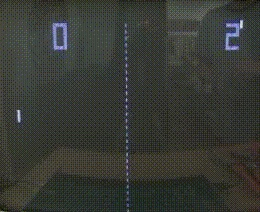
\includegraphics[scale=0.9]{images/Pong_Game_Test2.jpg}}
    \caption{Pong Game}
    \label{fig:pong}
\end{figure}

To simulate this game, we will be using Shift Register and an Arduino which help multiplex the output of the LED's. The LED's will be arranged in a 1D array and the ball will be moving from one end to the other. The player will have to hit the ball back to the opponent. The player who misses the ball will lose the game. The game will be played for 3 rounds and the player who wins 2 rounds will be the winner.

\section{Shift Register}

Flip flops can be used to store a single bit of binary data (1 or 0). However, in order to store multiple bits of data, we need multiple flip flops. N flip flops are to be connected in an order to store n bits of data. A Register is a device which is used to store such information. It is a group of flip flops connected in series used to store multiple bits of data. 

The information stored within these registers can be transferred with the help of shift registers. Shift Register is a group of flip flops used to store multiple bits of data. The bits stored in such registers can be made to move within the registers and in/out of the registers by applying clock pulses. An n-bit shift register can be formed by connecting n flip-flops where each flip flop stores a single bit of data.

Shift registers are basically of 4 types. These are:
\begin{itemize}
    \item Serial In, Serial Out (SISO)
    \item Serial In, Parallel Out (SIPO)
    \item Parallel In, Serial Out (PISO)
    \item Parallel In, Parallel Out (PIPO)
\end{itemize}

\subsection{D Flip Flop}

The D flip-flop is a clocked flip-flop with a single digital input 'D'. Each time a D flip-flop is clocked, its output follows the state of 'D'. The D Flip Flop has only two inputs D and CP. The D inputs go precisely to the S input and its complement is used to the R input.


Considering the pulse input is at 0, the outputs of gates 3 and 4 are at the 1 level and the circuit cannot convert state regardless of the value of D. The D input is sampled when CP = 1. If D is 1, the Q output goes to 1, locating the circuit in the set state. If D is 0, output Q goes to 0, and the circuit switches to a clear state.

\begin{figure}[h]
    \centering
    \subfloat[D Flip Flop]{
        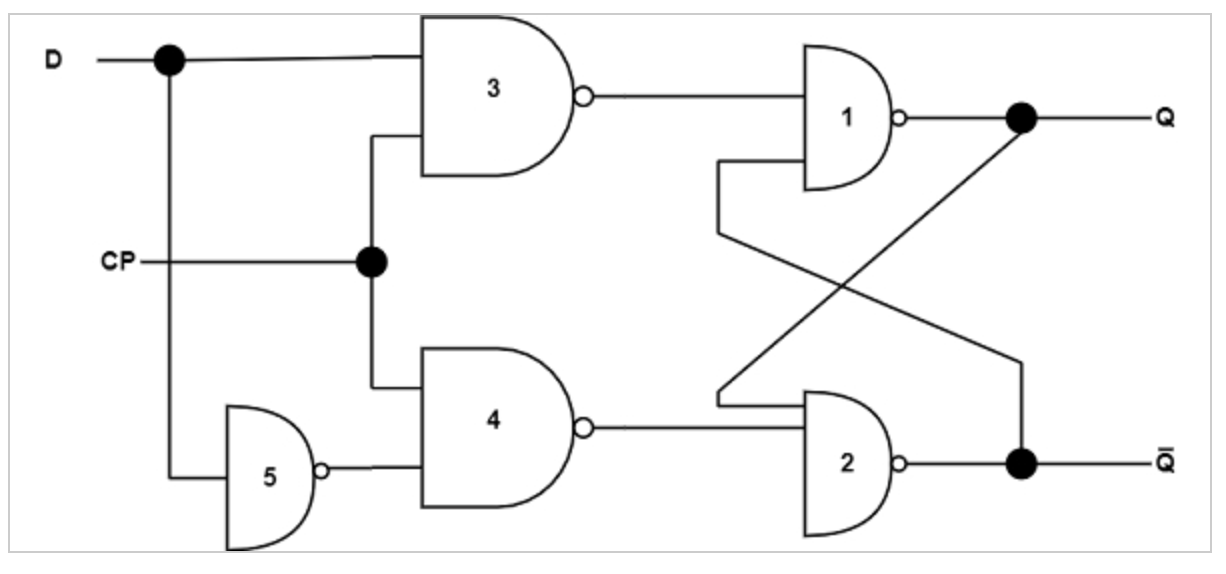
\includegraphics[width=0.5\textwidth]{images/D_Flip.png}
        \label{fig:d_flip_flop}
    }
    \subfloat[Truth Table]{
        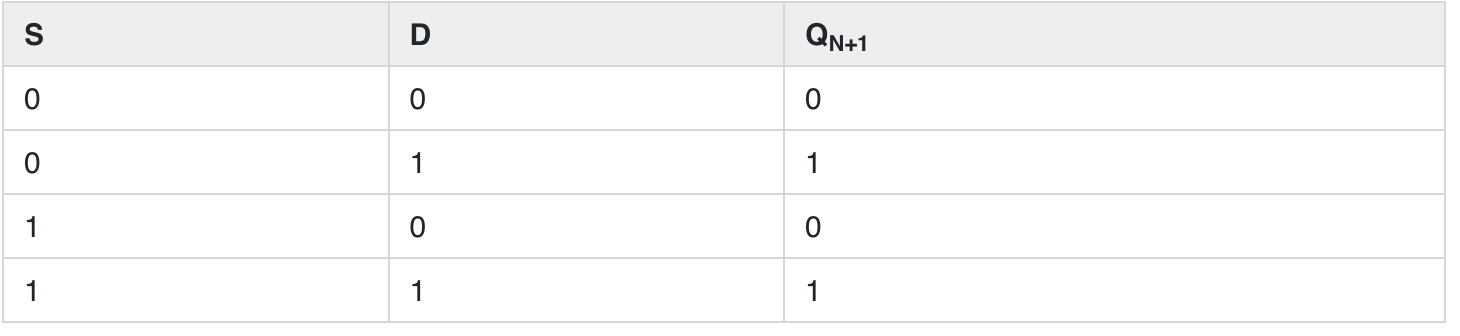
\includegraphics[width=0.5\textwidth]{images/D_truth.png}
        \label{fig:sr_flip_flop}
    }
    \caption{D Flip Flop}
\end{figure}

\chapter{Build Setup}
\section{Components Used}

\begin{itemize}
    \item \textbf{Arduino Uno}: Arduino board is a microcontroller kit for building digital devices.
    \item \textbf{IN74HC595A Shift Register}: Shift Register is a group of flip flops used to store multiple bits of data.
    \item \textbf{Breadboard}: A breadboard is a construction base used to build semi-permanent prototypes of electronic circuits
    \item \textbf{Jumper Wires}: A jumper wire is an electric wire that connects remote electric circuits used for printed circuit boards
    \item \textbf{LEDs}: A light-emitting diode (LED) is a semiconductor device that emits light when current flows through it
    \item \textbf{Resistors}: A resistor is a passive two-terminal electrical component that implements electrical resistance as a circuit element
\end{itemize}

\begin{figure}[H]
    \centering
    \subfloat[Arduino]{\label{fig:arduino}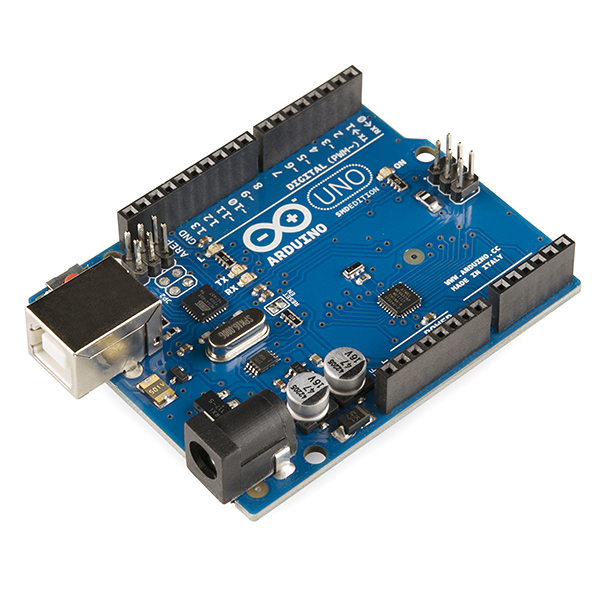
\includegraphics[width=.2\linewidth]{images/Arduino_Uno.jpg}}\hfill
    \subfloat[IN74HC595A]{\label{fig:IN74HC595A}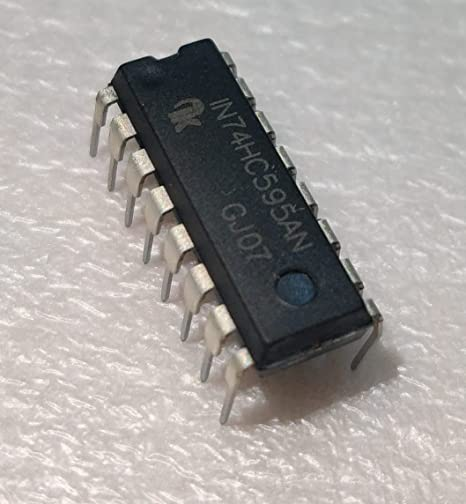
\includegraphics[width=.2\linewidth]{images/Shift_register.jpg}}\hfill
    \subfloat[Breadboard]{\label{fig:breadboard}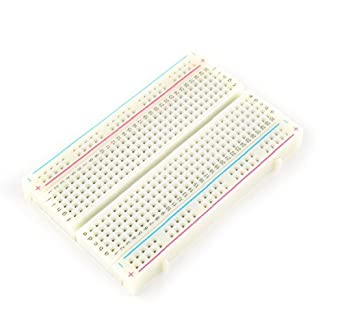
\includegraphics[width=.2\linewidth]{images/breadbaord.jpg}}\hfill
    \subfloat[LEDs]{\label{fig:leds}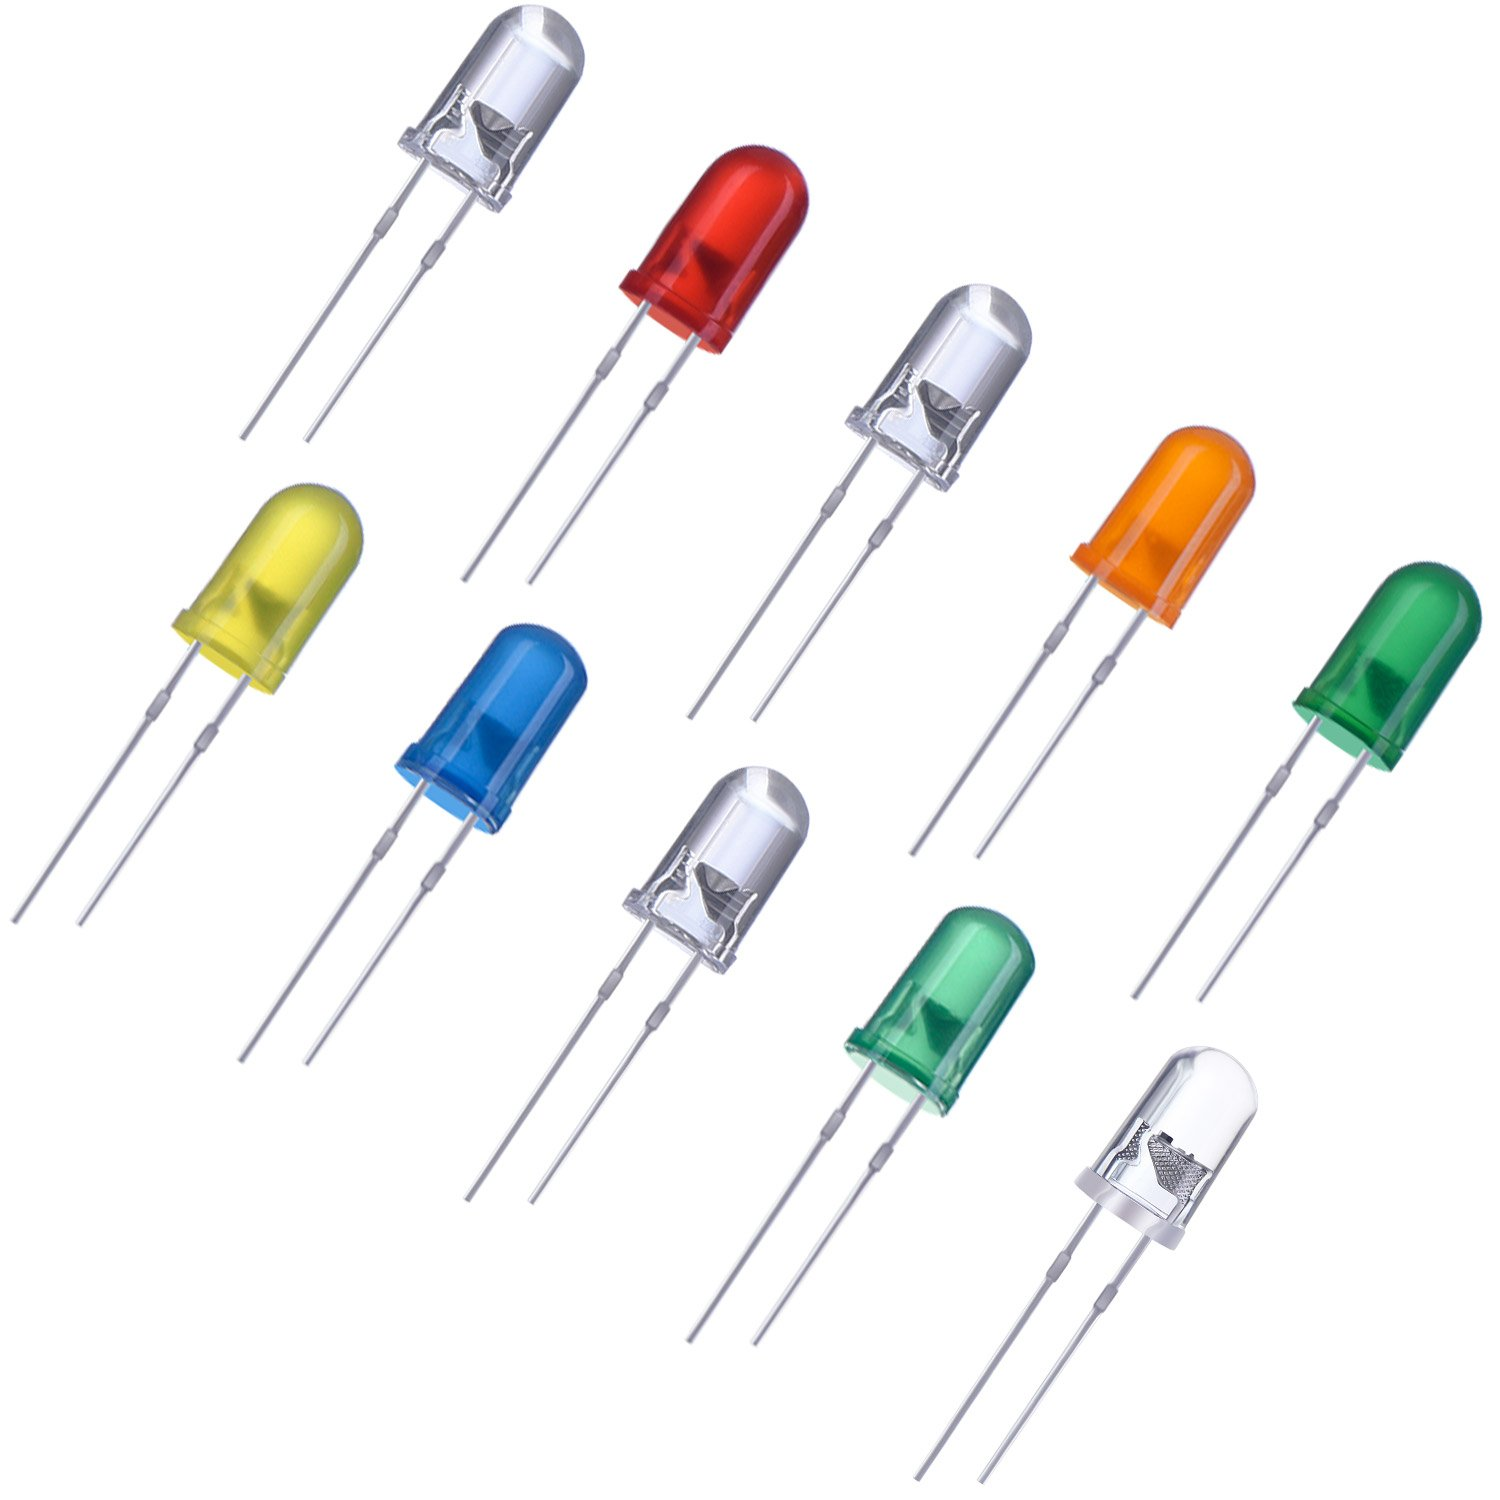
\includegraphics[width=.3\linewidth]{images/LEDs.jpg}}\par 
    \caption{Components Used}
    \label{fig: components}
\end{figure}

\section{Shift Register}

\textbf{IN74HC595A} is a 8-bit shift register. It has 8 output pins and 3 input pins. The 3 input pins are used to control the shift register. The 8 output pins are used to output the data stored in the shift register. The 3 input pins are as follows:
\begin{itemize}
    \item \textbf{Serial Data Input (DS)}: This pin is used to input the data to be stored in the shift register.
    \item \textbf{Shift Clock (SHCP)}: This pin is used to control the shifting of data in the shift register. When the clock is high, the data is shifted to the next flip flop. When the clock is low, the data is not shifted.
    \item \textbf{Store Clock (STCP)}: This pin is used to control the storing of data in the shift register. When the clock is high, the data is stored in the flip flop. When the clock is low, the data is not stored.
\end{itemize}

The other pins are:
\begin{itemize}
    \item \textbf{Serial Data Output (Q7)}: This pin is used to output the data stored in the last flip flop.
    \item \textbf{Master Reset (MR)}: This pin is used to reset the shift register. When the pin is high, the shift register is reset. When the pin is low, the shift register is not reset.
    \item \textbf{Output Enable (OE)}: This pin is used to enable the output of the shift register. When the pin is high, the output is enabled. When the pin is low, the output is disabled.
    \item \textbf{VCC}: This pin is used to supply power to the shift register.
    \item \textbf{GND}: This pin is used to supply ground to the shift register.
\end{itemize}

The IC can be used as a SIPO or a SISO shift register. The data is shifted one bit at a time when the shift clock is RISING edge triggered. Subsequently, when the latch clock is RISING edge triggered, the data is stored in the output pins. 


\begin{figure}[H]
    \centering
    \subfloat[IN74HC595A]{\label{fig:IN74HC595A}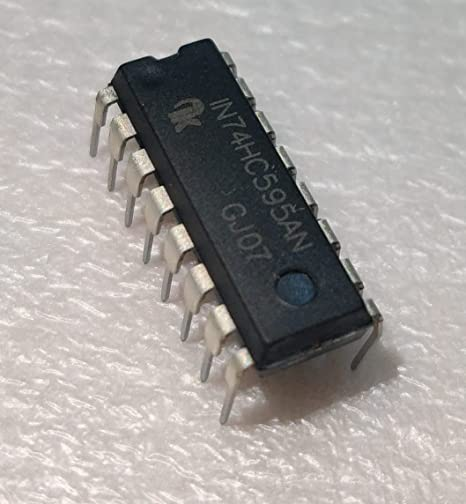
\includegraphics[width=.3\linewidth]{images/Shift_register.jpg}}\hfill
    \subfloat[Pin Diagram]{\label{fig:pin_diagram}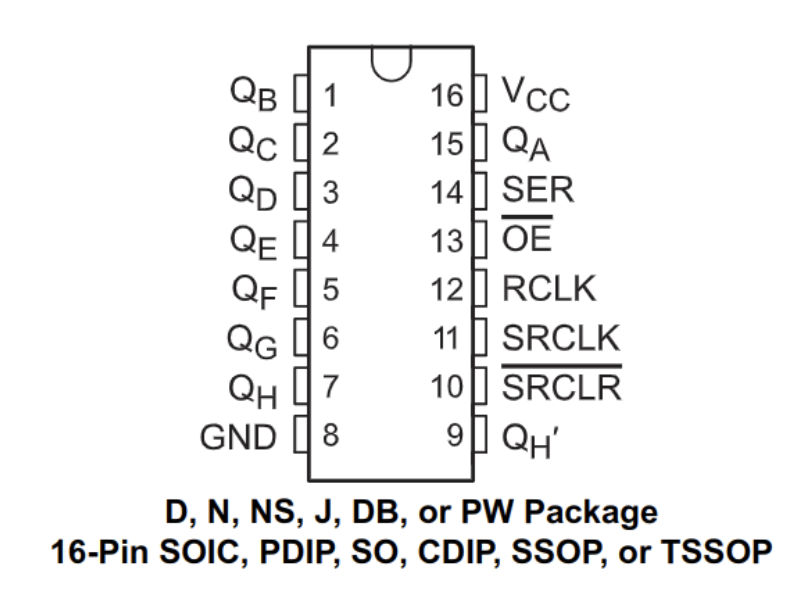
\includegraphics[width=.3\linewidth]{images/Pin_diagram.png}}\hfill
    \subfloat[Functional Diagram]{\label{fig: function_diagram}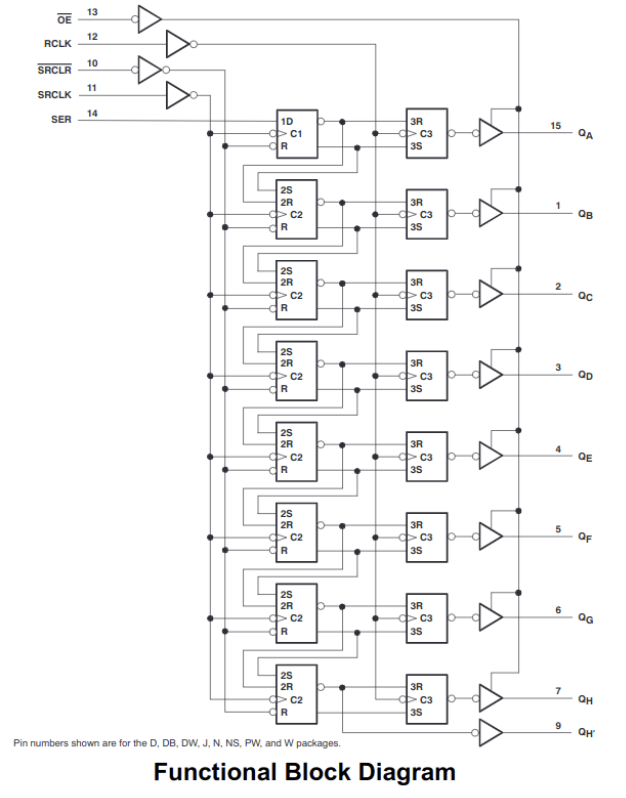
\includegraphics[width=.3\linewidth]{images/Functional_diagram.png}}\par 
    \caption{Shift Register}
    \label{fig: shift_register}
\end{figure}

The following is the signal flow and waveforms for the above mentioned pins:
\begin{figure}[h]
    \centering
    \subfloat[Signal Flow]{\label{fig:signal_flow}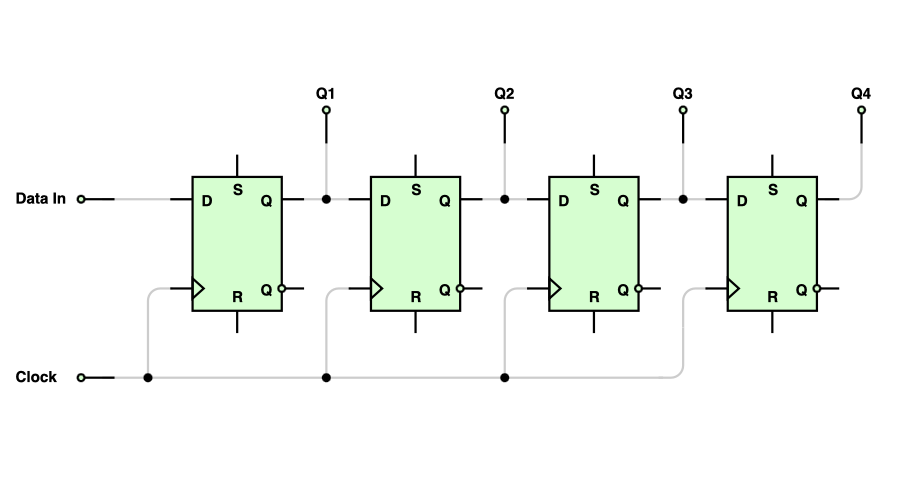
\includegraphics[width=.5\linewidth]{images/signal_flow.png}}\hfill
    \subfloat[Signal Waveform]{\label{fig: signal_waveform}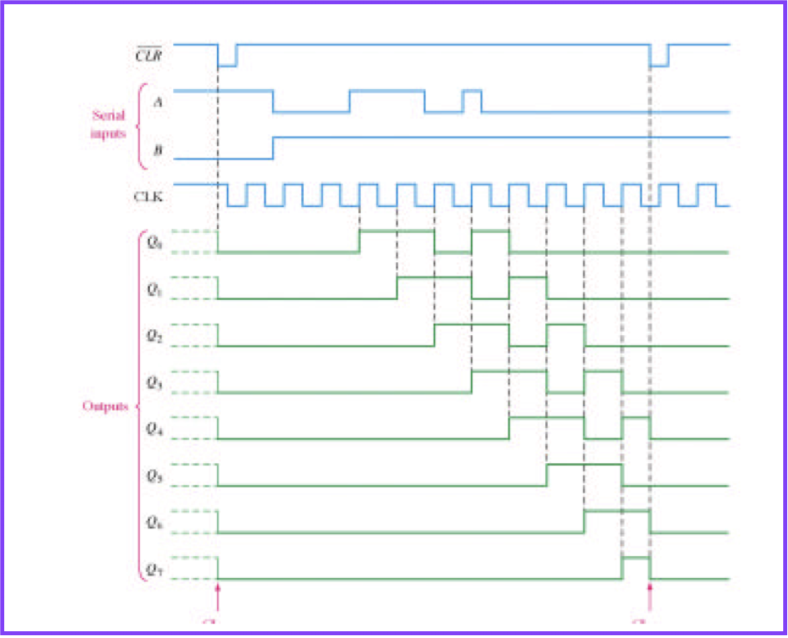
\includegraphics[width=.5\linewidth]{images/signal_waveform.png}}\par
    \caption{Signal Flow and Waveforms}
\end{figure}

\section{Arduino}

The Arduino Uno is a microcontroller board based on the ATmega328P. It has 14 digital input/output pins (of which 6 can be used as PWM outputs), 6 analog inputs, a 16 MHz crystal oscillator, a USB connection, a power jack, an ICSP header and a reset button. It contains everything needed to support the microcontroller; simply connect it to a computer with a USB cable or power it with a AC-to-DC adapter or battery to get started. It is programmed using the Arduino programming language (based on C++).

\begin{figure}[h]
    \centering
    \subfloat[Arduino Uno]{\label{fig:arduino}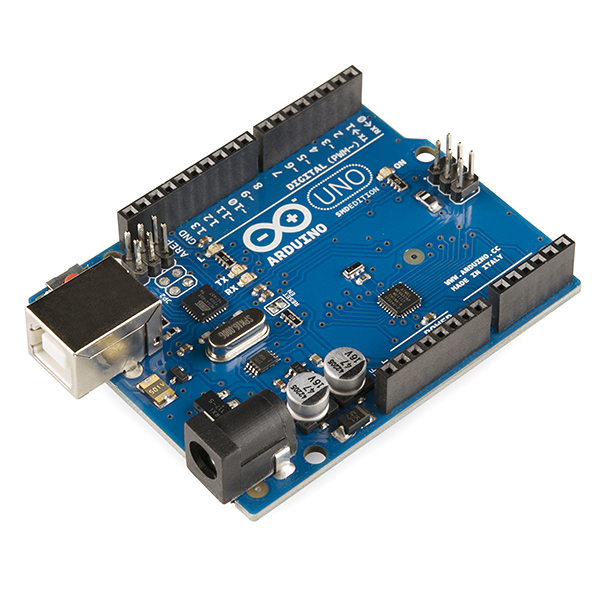
\includegraphics[width=.4\linewidth]{images/Arduino_Uno.jpg}}\hfill
    \subfloat[Pin Diagram]{\label{fig:pin_diagram}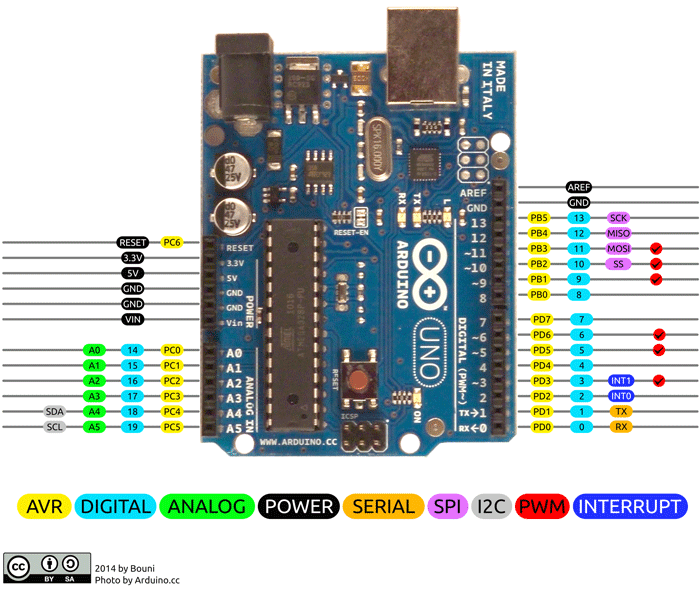
\includegraphics[width=.4\linewidth]{images/Arduino-Uno-Pin-Diagram.png}}\hfill
    \caption{Arduino Uno}
    \label{fig: arduino}
\end{figure}


\section{Circuit Diagram}

The followoing circuit diagram shows the connections between the components used in the project. The Arduino was connected to the shift register's data, clock and latch pins. The shift register's output pins were connected to the LED's. The LED's were connected in a 1D array.

\begin{figure}[H]
    \centering
    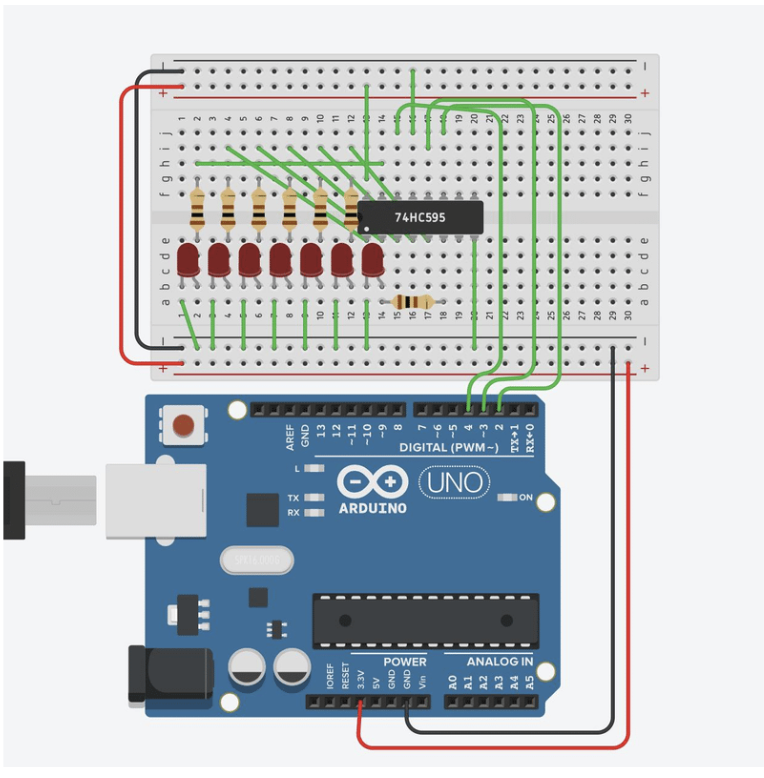
\includegraphics[width=.7\linewidth]{images/Circuit_diagram.png}
    \caption{Circuit Diagram}
    \label{fig: circuit}
\end{figure}

\section{Code}

The following code was used to control the shift register. The code was written in the Arduino IDE. The code was uploaded to the Arduino board. The code was written in C++.

\begin{lstlisting}[style=myArduino]

#include <Arduino.h>

const int datapin = 8;
const int clockpin = 9;
const int latchpin = 10;
const int button1_pin = 2;
const int button2_pin = 3;

// We'll also declare a global variable for the data we're // sending to the
// shift register:
byte data = 0;

int index = 0;
int direction = 1;
bool game_over = false;

volatile bool button1 = false, button2 = false;

void callback1() { button1 = true; };
void callback2() { button2 = true; };

void shiftWrite(int desiredPin, boolean desiredState)
{
    bitWrite(data, desiredPin, desiredState);
    shiftOut(datapin, clockpin, MSBFIRST, data);

    digitalWrite(latchpin, HIGH);
    digitalWrite(latchpin, LOW);
}

void setup()
{
    Serial.begin(9600);
    
    pinMode(datapin, OUTPUT);
    pinMode(clockpin, OUTPUT);
    pinMode(latchpin, OUTPUT);

    pinMode(button1_pin, INPUT_PULLUP);
    pinMode(button2_pin, INPUT_PULLUP);

    attachInterrupt(digitalPinToInterrupt(button1_pin), callback1, FALLING);
    attachInterrupt(digitalPinToInterrupt(button2_pin), callback2, FALLING);

    Serial.begin(9600);

    for (int i = 0; i < 8; i++)
    {
        shiftWrite(i, LOW);
    }
}

long cycles = 0;
bool cycle_flag = false;
long delay_time = 250;
void loop()
{
    if (!game_over)
    {
        if (index == 1 && button1 == true){
            direction = 1;
            cycles++;
            cycle_flag = true;

        }
        if (index == 6 && button2 == true){
            direction = -1;
            cycles++;
            cycle_flag = true;
        }

        button1 = false;
        button2 = false;

        if (cycle_flag && cycles % 2 == 0)
        {
            delay_time = max(5l, static_cast<long>(delay_time * 0.85));
            cycle_flag = false;
        }

        Serial.print(delay_time);
        Serial.print(" ");
        Serial.print(cycles);
        Serial.print(" ");
        index += direction;
        shiftWrite(index, HIGH);
        shiftWrite((index - direction), LOW);

        if (index == 0 || index == 7)
        {
            game_over = true;
            return;
        }
        Serial.println(index);
        delay(delay_time);
    }
    else
    {
        for (int i = 0; i < 8; i++)
            shiftWrite(i, HIGH);
        delay(100);
        for (int i = 0; i < 8; i++)
            shiftWrite(i, LOW);
        delay(100);
    }
}

\end{lstlisting}

\section{Results}

The circuit was assembled and the code was uploaded to the Arduino board. The following image shows the results of the project. 
The video of the project can be found at the following link: \url{https://drive.google.com/file/d/1isGdwd_6Z0JKoO3FJOv7HLgnDQ60ZBAJ/view?usp=share_link}

\begin{figure}[h]
    \centering
    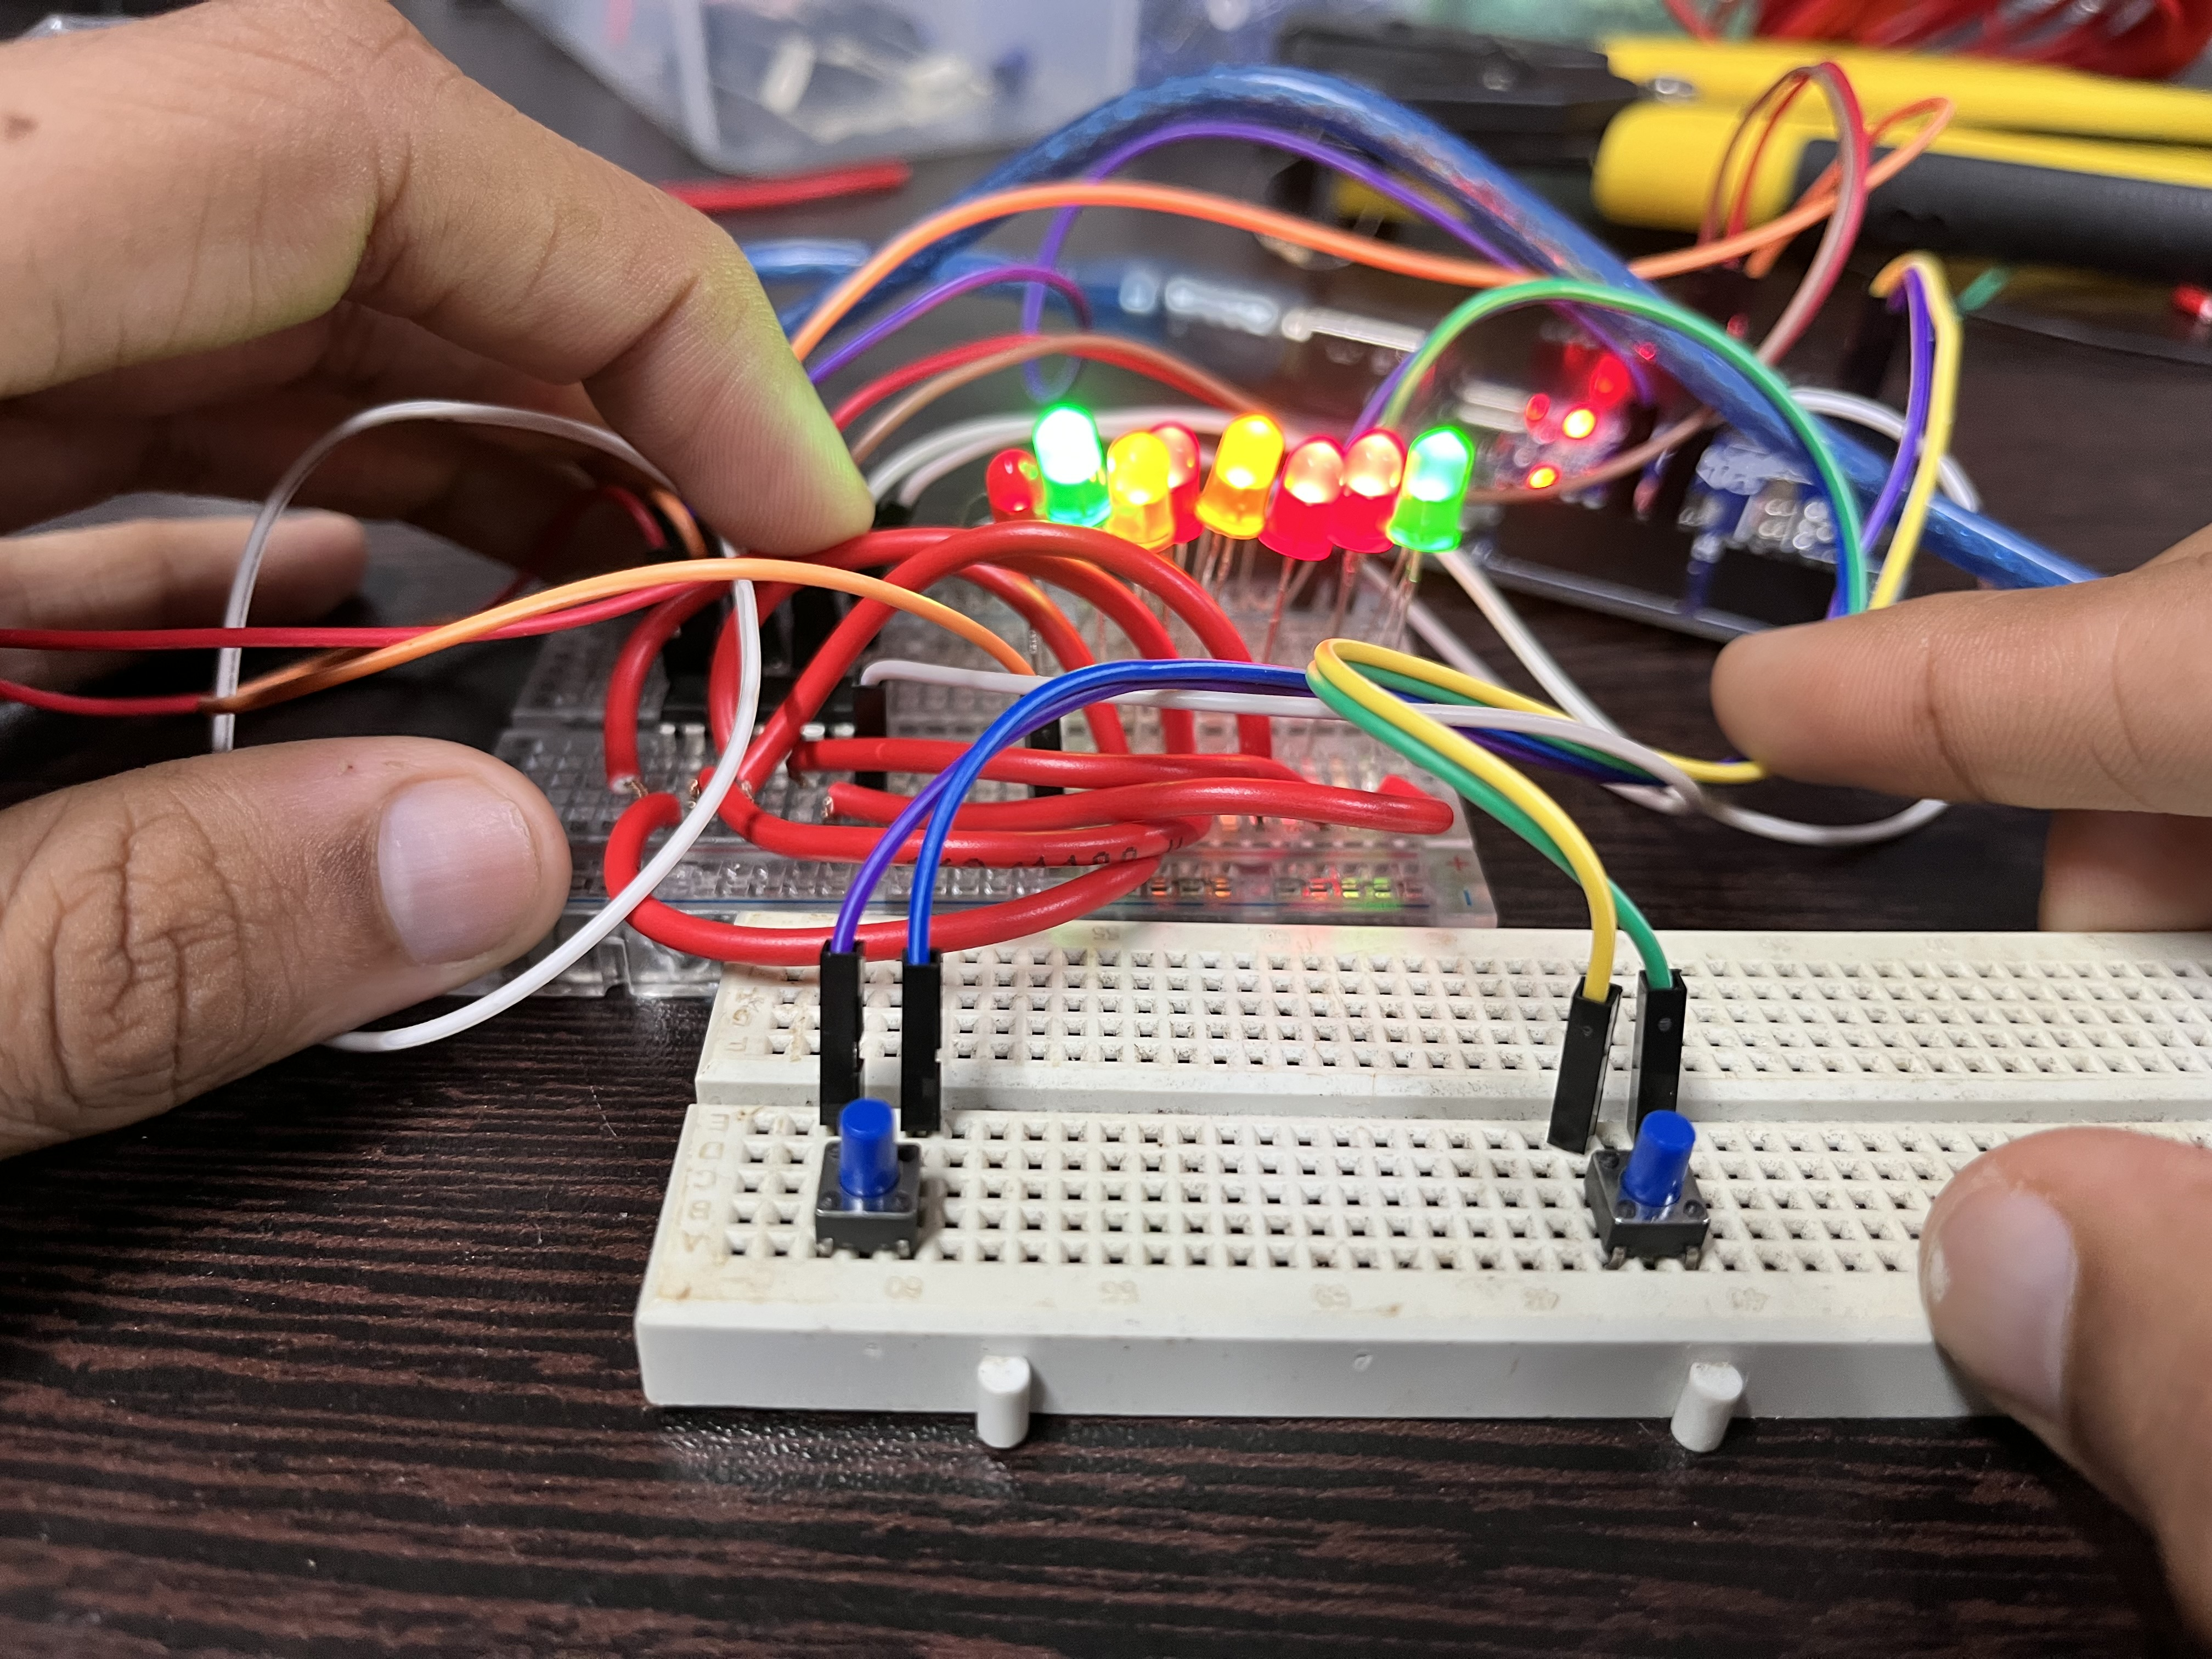
\includegraphics[width=.7\textwidth]{images/LED_result.jpeg}
    \caption{Results}
    \label{fig: results}
\end{figure}





\chapter{Conclusion}

We have successfully developed an LED Ping Pong game using a Shift Register and an Arduino.

\end{document}


